% Copyright (c) 2022 by Lars Spreng
% This work is licensed under the Creative Commons Attribution 4.0 International License.

\documentclass[
11pt,notheorems,hyperref={pdfauthor=whatever}
]{beamer}

\usepackage{kotex}
\input{loadslides.tex}

\usepackage{fontspec}
\IfFileExists{/Users/seojunha/Library/Fonts/NotoSansCJKkr-Regular.otf}{%
  \setmainhangulfont[
    Path=/Users/seojunha/Library/Fonts/,
    BoldFont=NotoSansCJKkr-Bold.otf
  ]{NotoSansCJKkr-Regular.otf}
  \setsanshangulfont[
    Path=/Users/seojunha/Library/Fonts/,
    BoldFont=NotoSansCJKkr-Bold.otf
  ]{NotoSansCJKkr-Regular.otf}
  \setmonohangulfont[
    Path=/Users/seojunha/Library/Fonts/,
    BoldFont=NotoSansCJKkr-Bold.otf
  ]{NotoSansCJKkr-Regular.otf}
}{%
  \IfFontExistsTF{Noto Sans CJK KR}{%
    \setmainhangulfont{Noto Sans CJK KR}
    \setsanshangulfont{Noto Sans CJK KR}
    \setmonohangulfont{Noto Sans CJK KR}
  }{%
    \IfFontExistsTF{NanumGothic}{%
      \setmainhangulfont{NanumGothic}
      \setsanshangulfont{NanumGothic}
      \setmonohangulfont{NanumGothic}
    }{}%
  }%
}
\renewcommand{\familydefault}{\sfdefault}

\definecolor{TextGray}{HTML}{333333}
\definecolor{AccentOrange}{HTML}{08457E}
\definecolor{SoftOrange}{HTML}{EAF0F8}
\definecolor{LineGray}{HTML}{B8B8B8}

\usepackage{tikz}
\usetikzlibrary{arrows.meta, positioning, fit, backgrounds, calc, shapes.geometric}

\addtobeamertemplate{frametitle}{}{\vspace{-0.5em}}

\tikzset{
  box/.style={draw=LineGray, rounded corners=2pt, fill=white, align=center, minimum height=0.82cm, inner sep=5pt, font=\small},
  orangebox/.style={draw=AccentOrange, very thick, rounded corners=2pt, fill=SoftOrange, align=center, minimum height=0.82cm, inner sep=5pt, font=\small\bfseries},
  arrow/.style={-{Latex[length=2.6mm]}, thick, draw=AccentOrange},
  grayarrow/.style={-{Latex[length=2.4mm]}, thick, draw=LineGray}
}

\newcommand{\smallgray}[1]{{\scriptsize\textcolor{gray!75}{#1}}}
\newcommand{\smallred}[1]{{\scriptsize\textcolor{red!70!black}{#1}}}
\newcommand{\tagbox}[1]{\colorbox{SoftOrange}{\strut\scriptsize #1}}
\newcommand{\yes}{\textcolor{TextGray}{Yes}}
\newcommand{\no}{\textcolor{TextGray}{No}}

\setbeamerfont{title}{size=\LARGE,series=\bfseries}
\setbeamerfont{subtitle}{size=\normalsize}
\setbeamerfont{frametitle}{series=\bfseries}

\title[]{MIMIC-CDM 기반 Sequential Clinical Diagnosis 연구 동향}
\subtitle{Path Supervision과 Stopping 문제를 중심으로}
\author[]{하서준}
\institute{DGIST}
\date{2026년 5월 22일}

\begin{document}

{
\setbeamertemplate{footline}{}
\begin{frame}
  \titlepage
  \vspace{-0.8em}
  \begin{center}
  \scriptsize
  LA-CDM · LDTL · SIFT · CaRT · MIMIC-CDM
  \end{center}
\end{frame}
}
\addtocounter{framenumber}{-1}

\begin{frame}{Survey Map}
\vspace{0.45em}
\begin{center}
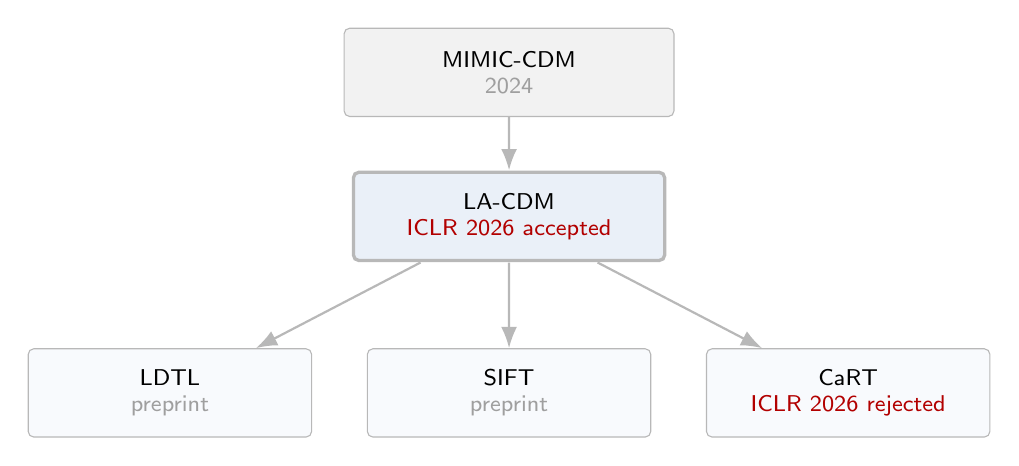
\begin{tikzpicture}[scale=1.18, transform shape,
  paper/.style={draw=LineGray, rounded corners=2pt, fill=white, align=center, minimum width=3.05cm, minimum height=0.95cm, font=\scriptsize},
  root/.style={paper, fill=gray!10, minimum width=3.55cm},
  hub/.style={paper, draw=LineGray, very thick, fill=SoftOrange, minimum width=3.35cm},
  axis/.style={font=\scriptsize\bfseries, text=TextGray}
]
\node[root] (data) at (0,0) {MIMIC-CDM\\\smallgray{2024}};
\node[hub] (lacdm) at (0,-1.55) {LA-CDM\\\smallred{ICLR 2026 accepted}};
\node[paper, fill=SoftOrange!35] (ldtl) at (-3.65,-3.45) {LDTL\\\smallgray{preprint}};
\node[paper, fill=SoftOrange!35] (sift) at (0,-3.45) {SIFT\\\smallgray{preprint}};
\node[paper, fill=SoftOrange!35] (cart) at (3.65,-3.45) {CaRT\\\smallred{ICLR 2026 rejected}};

\draw[-{Latex[length=2.7mm]}, thick, draw=LineGray] (data) -- (lacdm);
\draw[-{Latex[length=2.7mm]}, thick, draw=LineGray] (lacdm) -- (ldtl);
\draw[-{Latex[length=2.7mm]}, thick, draw=LineGray] (lacdm) -- (sift);
\draw[-{Latex[length=2.7mm]}, thick, draw=LineGray] (lacdm) -- (cart);
\end{tikzpicture}
\end{center}
\vspace{-0.1em}
\begin{block}{최근에 생긴 문제 세팅}
\small
MIMIC-CDM (2024)이 \textbf{sequential evidence acquisition}을 benchmark로 만들면서,
LLM diagnosis가 ``full information classification''에서 ``어떤 검사를 언제 볼 것인가''를 학습하는 문제로 이동했다.
\end{block}
\end{frame}

\begin{frame}{오늘의 발표 흐름}
\vspace{0.1em}
\begin{enumerate}
\small
  \item \textbf{LA-CDM}: MIMIC-CDM에서 RL clinical decision making을 어떻게 문제화했는가
  \item \textbf{LDTL}: path label 부재를 local information gain으로 어떻게 우회했는가
  \item \textbf{SIFT}: terminal reward 대신 critical evidence reward를 어떻게 만들었는가
  \item \textbf{Combination 관점}: 검사 조합의 utility를 직접 보면 무엇이 달라지는가
  \item \textbf{OpenReview}: LA-CDM은 어떤 약점에도 불구하고 왜 accepted 되었는가
\end{enumerate}

\vspace{0.55em}
\begin{block}{발표의 중심 질문}
\small
정답 diagnosis label은 있지만 \textbf{좋은 diagnostic path label은 없다}. 기존 논문들은 이 빈칸을 어떤 proxy로 메우고 있는가?
\end{block}
\end{frame}

\begin{frame}[plain]
\centering
\vspace{0.22\textheight}
{\Large\bfseries Language Agents for Hypothesis-driven\\Clinical Decision Making with Reinforcement Learning}
\vspace{1.2em}

{\small LA-CDM}\\
{\scriptsize ICLR 2026}
\end{frame}

\begin{frame}{LA-CDM: 문제 제기}
\vspace{0.1em}
\begin{block}{1. 기존 clinical RL은 주로 tabular data만 고려함}
\small
기존 reinforcement learning 기반 clinical decision-making은 주로 \textbf{tabular data}에 맞춰져 있다. 그래서 clinical notes, imaging reports처럼 실제 진단에서 중요한 modality를 놓친다.
\end{block}

\vspace{0.55em}
\begin{block}{2. 기존 LLM clinical decision-making은 대부분 zero-shot임}
\small
기존 LLM 기반 clinical decision-making은 prompting이나 zero-shot reasoning에 의존한다. 즉, \textbf{diagnostic test selection과 sequential decision-making 자체를 명시적으로 학습}하지 않는다.
\end{block}

\vspace{0.55em}
\begin{block}{LA-CDM의 문제 설정}
\small
그래서 LA-CDM은 multimodal patient state에서 test를 순차적으로 요청하고, confidence가 충분할 때 diagnosis를 내리는 LLM-based clinical decision-making 문제를 제시한다.
\end{block}
\end{frame}

\begin{frame}[t]{LA-CDM: Main Figure}
\centering
\vspace{0.35em}
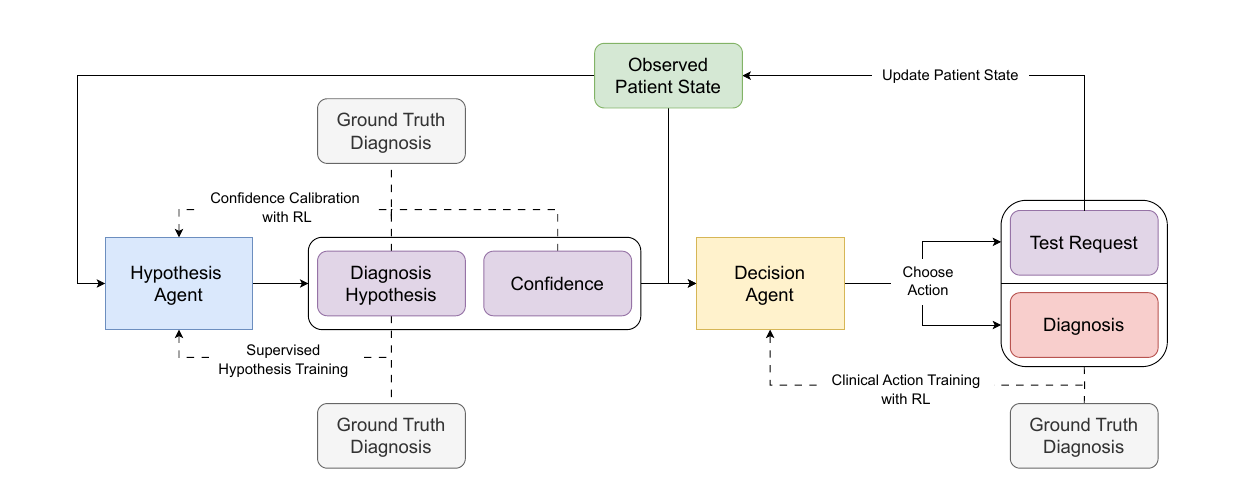
\includegraphics[width=0.98\linewidth,height=0.78\textheight,keepaspectratio]{figures/LA-CDM/main.png}
\end{frame}

\begin{frame}{LA-CDM: 방법}
\vspace{0.1em}
\begin{center}
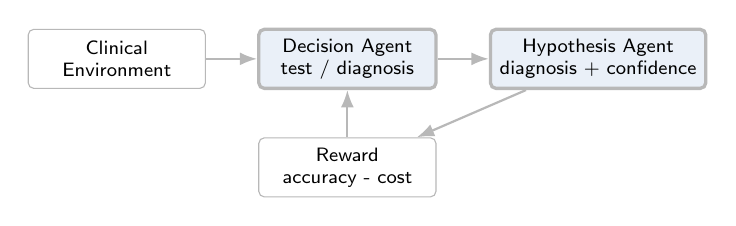
\begin{tikzpicture}[
  box/.style={draw=LineGray, rounded corners=2pt, fill=white, align=center, minimum width=2.25cm, minimum height=0.75cm, font=\scriptsize},
  train/.style={box, draw=LineGray, very thick, fill=SoftOrange},
  arr/.style={-{Latex[length=2.2mm]}, thick, draw=LineGray}
]
\node[box] (env) {Clinical\\Environment};
\node[train, right=0.65cm of env] (da) {Decision Agent\\test / diagnosis};
\node[train, right=0.65cm of da] (ha) {Hypothesis Agent\\diagnosis + confidence};
\node[box, below=0.6cm of da] (reward) {Reward\\accuracy - cost};
\draw[arr] (env) -- (da);
\draw[arr] (da) -- (ha);
\draw[arr] (ha) -- (reward);
\draw[arr] (reward) -- (da);
\end{tikzpicture}
\end{center}

\vspace{0.35em}
\begin{columns}[T,onlytextwidth]
\begin{column}{0.48\textwidth}
\begin{block}{Cyclic training objectives}
\footnotesize
\begin{enumerate}
  \item \textbf{Hypothesis generation}\\
  HA가 각 state에서 정답 diagnosis \(y_{\mathrm{true}}\)를 생성하도록 SFT.
  \item \textbf{Uncertainty-awareness}\\
  confidence가 \(J(h_j)=\mathbb{1}[h_j=y_{\mathrm{true}}]\)에 맞도록 GRPO calibration.
  \item \textbf{Efficient action selection}\\
  DA가 필요한 test와 stop/diagnosis를 GRPO로 학습.
\end{enumerate}
\end{block}
\end{column}
\begin{column}{0.48\textwidth}
\begin{block}{DA phase reward}
\small
\[
R_{\mathrm{diag}}=
\begin{cases}
r_{\mathrm{pos}} & y_{\mathrm{pred}}=y_{\mathrm{true}}\\
r_{\mathrm{neg}} & y_{\mathrm{pred}}\neq y_{\mathrm{true}}\\
r_{\mathrm{invalid}} & \text{format error}
\end{cases}
\]
\vspace{-0.4em}
\[
R_{\mathrm{cost}}(T)=-\sum_{t_j\in T}c(t_j)
\]
\vspace{-0.1em}
\footnotesize
이 reward는 \textbf{efficient action selection phase}에서만 쓰인다. Hypothesis SFT와 confidence calibration은 별도 objective로 cycle 안에서 번갈아 학습된다.
\end{block}
\end{column}
\end{columns}
\end{frame}

\begin{frame}[t]{LA-CDM: 결과와 의미}
\centering
\vspace{0.7em}
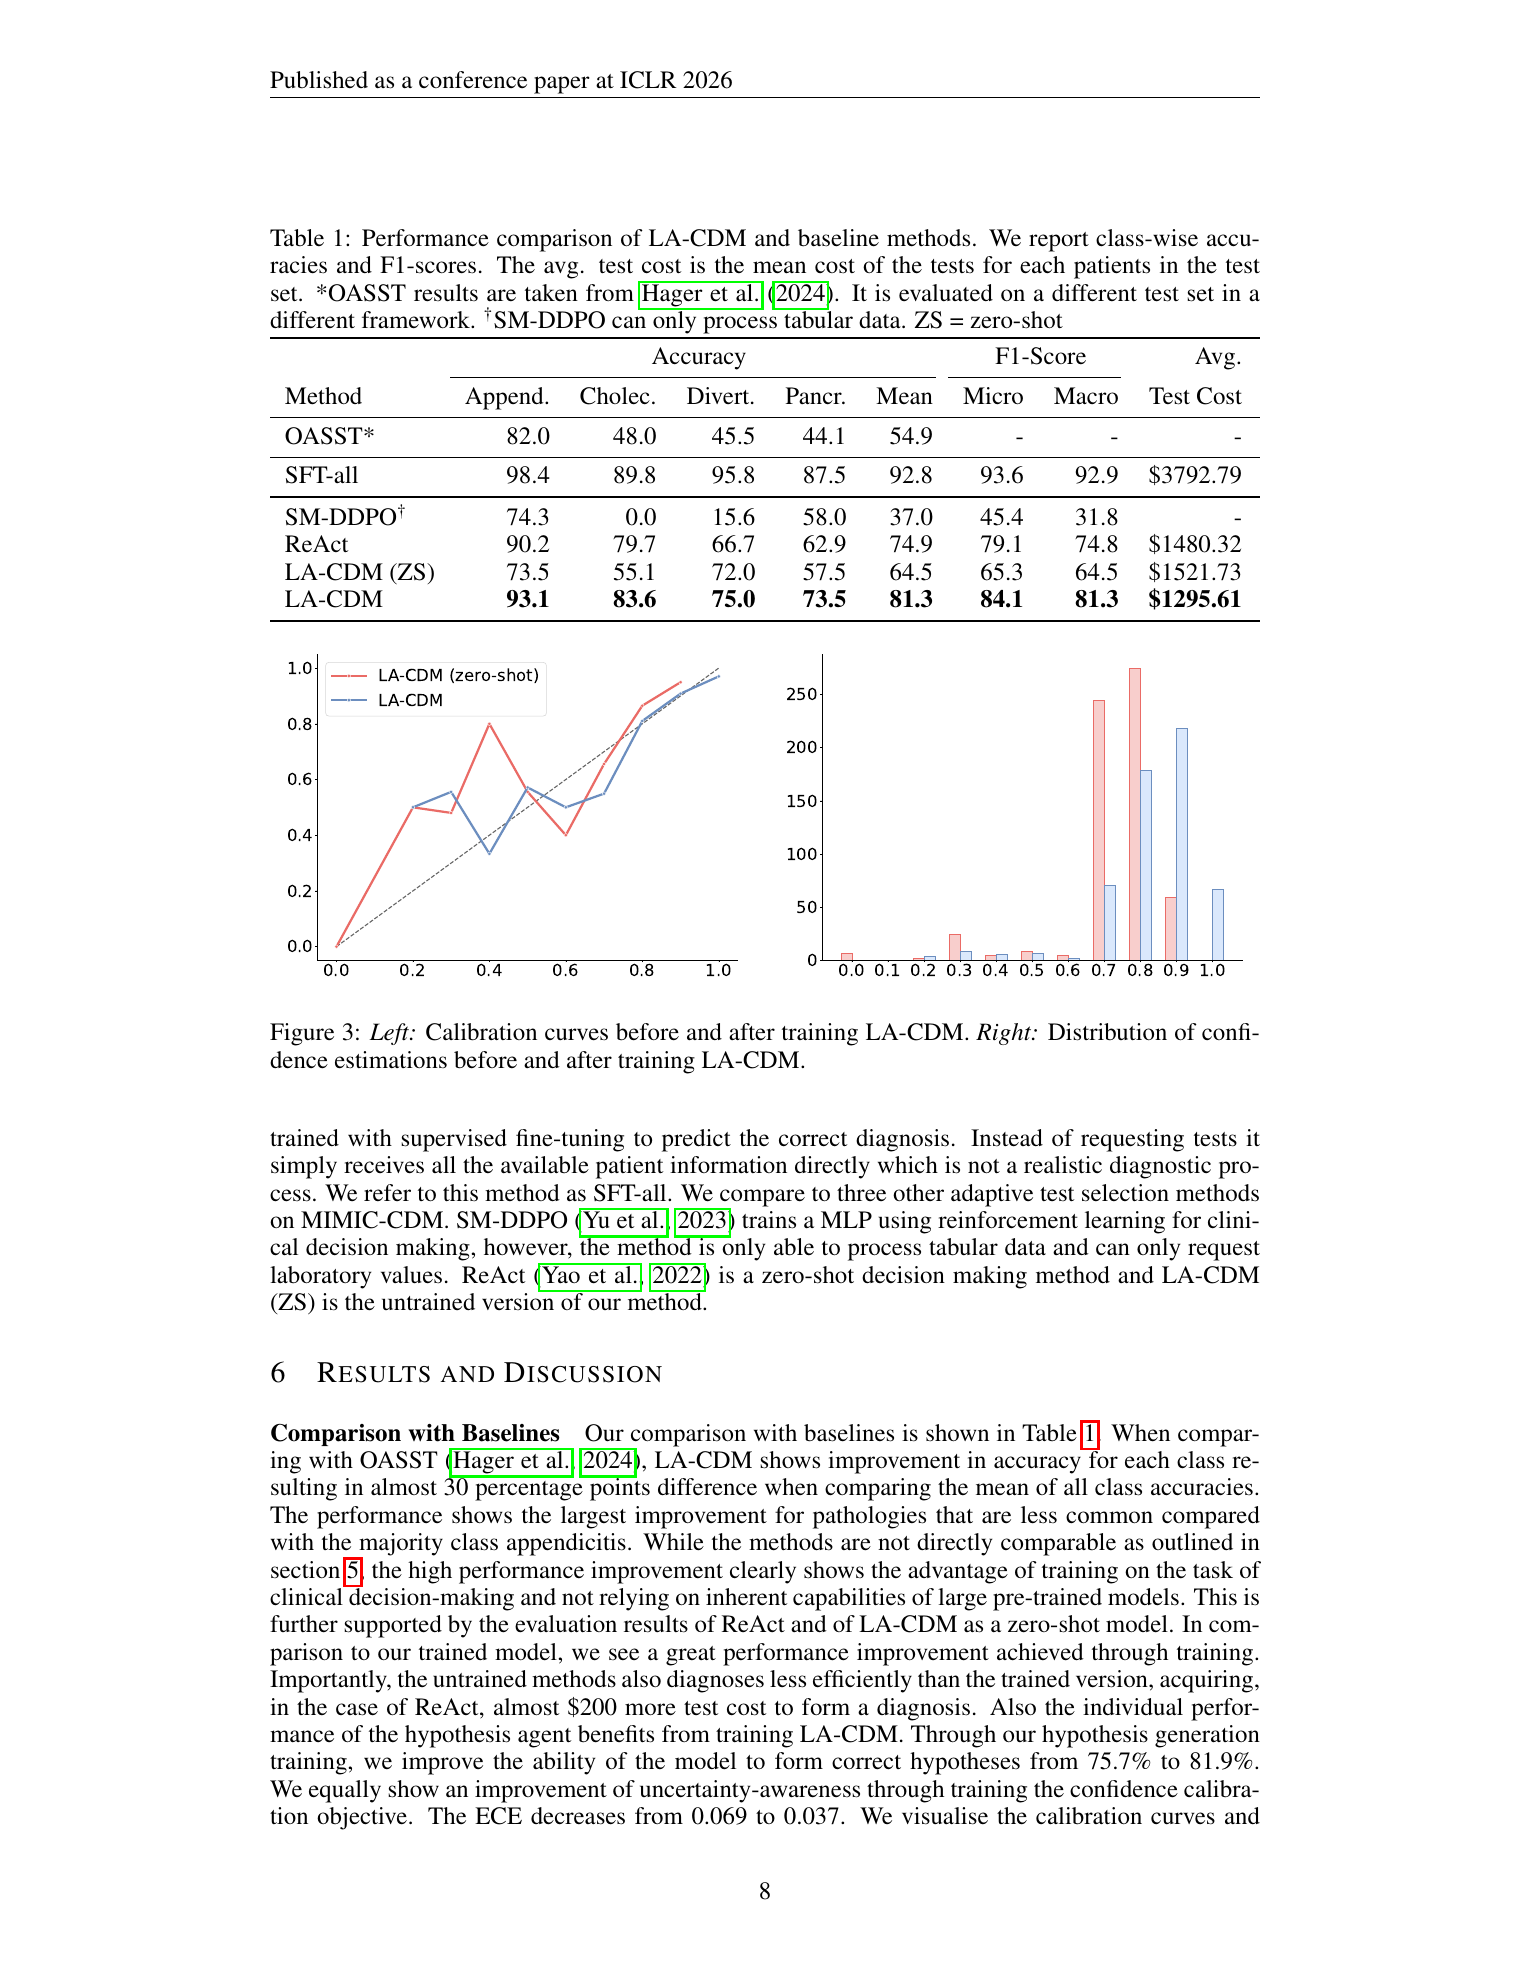
\includegraphics[
  width=0.96\linewidth,
  height=0.58\textheight,
  keepaspectratio,
  trim=3.2cm 14.0cm 2.6cm 4.9cm,
  clip
]{figures/LA-CDM/results/page-08.png}

\vspace{0.2em}
\begin{block}{결과가 주장하는 것}
\small
\begin{itemize}
  \item LA-CDM mean accuracy \(81.3\), macro F1 \(81.3\)
  \item ReAct보다 높은 성능과 낮은 평균 test cost
  \item training 후 confidence calibration도 개선
\end{itemize}
\end{block}
\end{frame}

\begin{frame}[plain]
\centering
\vspace{0.22\textheight}
{\Large\bfseries Uncertainty-Guided Latent Diagnostic\\Trajectory Learning for Sequential Clinical Diagnosis}
\vspace{1.2em}

{\small LDTL}\\
{\scriptsize arXiv 2026}
\end{frame}

\begin{frame}{LDTL: 문제 제기}
\vspace{0.1em}
\begin{block}{1. LLM 진단은 test selection을 명시적으로 모델링하지 못함}
\small
LLM 기반 diagnostic system은 진단을 생성할 수는 있지만, 실제 임상 경로처럼 \textbf{어떤 test를 어떤 순서로 선택해야 하는지}를 명시적으로 모델링하지 못한다.
\end{block}

\vspace{0.35em}
\begin{block}{2. Terminal reward만으로는 trajectory 학습이 부족함}
\small
terminal reward로 성능과 비용을 최적화하는 방식은 \textbf{diagnostic trajectory의 구조나 분포}를 직접 제어하지 못한다. 따라서 제한된 clinical trajectories에서 불안정하고, 어떤 path가 바람직한지에 대한 supervision이 약하다.
\end{block}

\vspace{0.35em}
\begin{block}{LDTL의 문제 설정}
\small
그래서 LDTL은 test selection을 \textbf{Latent Diagnostic Trajectory Learning} 문제로 두고, 단순 reward가 아니라 diagnostic improvement 기반의 action signal을 만들려고 한다.
\end{block}
\end{frame}

\begin{frame}[t]{LDTL: Main Figure}
\centering
\vspace{0.35em}

\includegraphics[width=0.98\linewidth,height=0.78\textheight,keepaspectratio]{figures/LDTL/main.png}
\end{frame}

\begin{frame}[t]{LDTL: ideal vs. approximation}
\vspace{0.85em}
\begin{columns}[T,onlytextwidth]
\begin{column}{0.48\textwidth}
{\large\bfseries\textcolor{primary}{Ideal: trajectory posterior}}

\vspace{0.25em}
{\small
\[
q(z \mid h_0, y) =
\frac{\exp(\beta S(z))}
{\sum_{z' \in Z(h_0)} \exp(\beta S(z'))}
\]
\[
q(a_t \mid h_t, y) =
\sum_{z:z_t=a_t} q(z \mid h_0, y)
\]
}

\vspace{-0.55em}
\begin{center}
\scriptsize
\begin{tabular}{lcc}
\toprule
trajectory \(z\) & \(S(z)\) & \(q(z)\) \\
\midrule
\((A,B,C)\) & 3.0 & 0.30 \\
\((A,C,B)\) & 2.0 & 0.12 \\
\((B,A,C)\) & 2.5 & 0.20 \\
\((B,C,A)\) & 3.5 & 0.35 \\
\((C,A,B)\) & 1.0 & 0.02 \\
\((C,B,A)\) & 0.5 & 0.01 \\
\bottomrule
\end{tabular}
\end{center}

\vspace{-0.45em}
{\small
\[
q(A)=0.42,\quad q(B)=0.55,\quad q(C)=0.03
\]
}

{\scriptsize \(B\) 단독 gain이 작아도, \(B\)로 시작하는 좋은 future trajectory가 많으면 \(B\)가 선택된다.}
\end{column}

\begin{column}{0.02\textwidth}
\centering
\vspace{0.05em}
\rule{0.4pt}{0.70\textheight}
\end{column}

\begin{column}{0.48\textwidth}
{\large\bfseries\textcolor{primary}{Approx.: one-step IG}}

\vspace{0.25em}
{\small
\[
IG(h_0,a)=\log p(y\mid h_0+a)-\log p(y\mid h_0)
\]
\[
q(a\mid h_0,y)\propto \exp(IG(h_0,a)/\tau)
\]
}

\vspace{-0.35em}
\begin{center}
\scriptsize
\begin{tabular}{lc}
\toprule
action & one-step IG \\
\midrule
\(A\) & 0.70 \\
\(B\) & 0.50 \\
\(C\) & 0.10 \\
\bottomrule
\end{tabular}
\end{center}

\vspace{0.15em}
{\small
\[
IG(A)>IG(B)>IG(C)
\]
}

{\scriptsize 실제 근사는 \(A\)를 더 선호한다. 하지만 \(B\rightarrow C\rightarrow A\)처럼 최종 utility가 큰 조합은 명시적으로 평가하지 않는다.}
\end{column}
\end{columns}
\end{frame}

\begin{frame}{LDTL: approximation gap}
\vspace{0.35em}
\begin{block}{Trajectory marginal을 전개하면}
\small
현재 action 이후의 future trajectory를 \(\tau\)라고 두면 \(z=(a,\tau)\)이다.
\[
q(a\mid h_t,y)
\propto
\sum_{\tau}\exp\!\left(\beta S(a,\tau)\right)
\]
\end{block}

\vspace{0.35em}
\begin{block}{만약 trajectory score가 immediate gain과 future utility로 나뉜다면}
\small
\[
S(a,\tau)=IG(h_t,a)+S_{\mathrm{future}}(\tau\mid h_t,a)
\]
\[
q(a\mid h_t,y)
\propto
\exp(\beta IG(h_t,a))
\underbrace{\sum_{\tau}\exp\!\left(\beta S_{\mathrm{future}}(\tau\mid h_t,a)\right)}_{Z_{\mathrm{future}}(h_t,a)}
\]
\end{block}

\vspace{0.35em}
\begin{alertblock}{LDTL approximation이 생략하는 항}
\small
LDTL의 one-step IG posterior는 \(Z_{\mathrm{future}}(h_t,a)\)를 계산하지 않는다. 이 근사가 맞으려면 \(Z_{\mathrm{future}}(h_t,a)\)가 action마다 거의 같아야 한다.
\end{alertblock}
\end{frame}

\begin{frame}{LDTL: 방법}
\vspace{0.05em}
\begin{block}{Stage 1. Diagnostic LLM을 먼저 학습}
\small
full patient information, 즉 complete diagnostic results가 주어졌을 때 correct disease label을 예측하고 confidence score를 출력하도록 diagnostic LLM을 SFT한다.
\end{block}

\vspace{0.45em}
\begin{block}{Stage 2. Diagnostic LLM은 freeze하고 planner를 학습}
\small
학습된 diagnostic LLM을 고정한 뒤, planning LLM이 어떤 diagnostic action을 선택할지 학습한다. 각 step에서 action을 넣어본 뒤 \textbf{diagnostic improvement}로 action-level posterior \(q(a_t\mid h_t,y)\)를 만들고, planner policy를 여기에 맞춘다.
\end{block}

\vspace{0.35em}
\[
\mathcal{L}_{\mathrm{planner}}
=
\sum_{t=1}^{T}
\mathrm{KL}\!\left(q(a\mid h_t,y)\,\|\,\pi_\theta(a\mid h_t)\right)
\]

\vspace{0.15em}
\begin{block}{핵심}
\small
정답 trajectory를 직접 만들지 않고, \textbf{freeze된 diagnostic LLM의 probability 변화}를 이용해서 planner supervision을 만든다.
\end{block}
\end{frame}

\begin{frame}[t]{LDTL: 결과와 의미}
\centering
\vspace{1.45em}
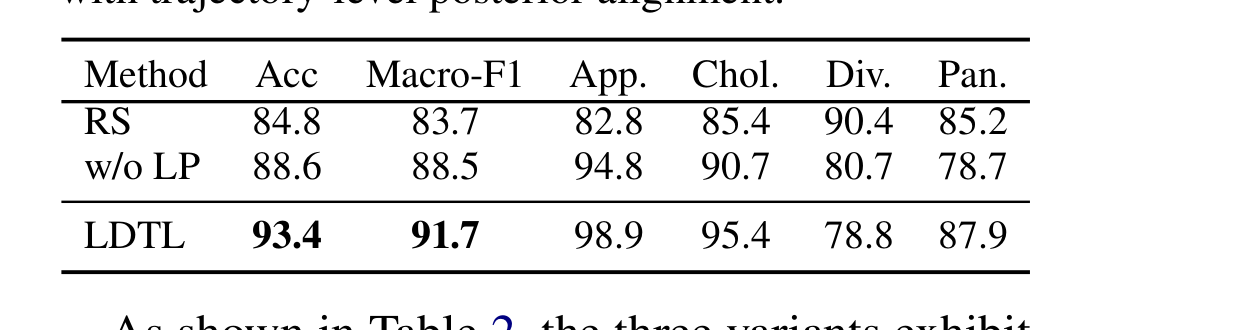
\includegraphics[
  width=0.96\linewidth,
  height=0.29\textheight,
  keepaspectratio,
  trim=0 0.25cm 0 0.45cm,
  clip
]{figures/LDTL/results/table2_crop.png}

\vspace{0.1em}
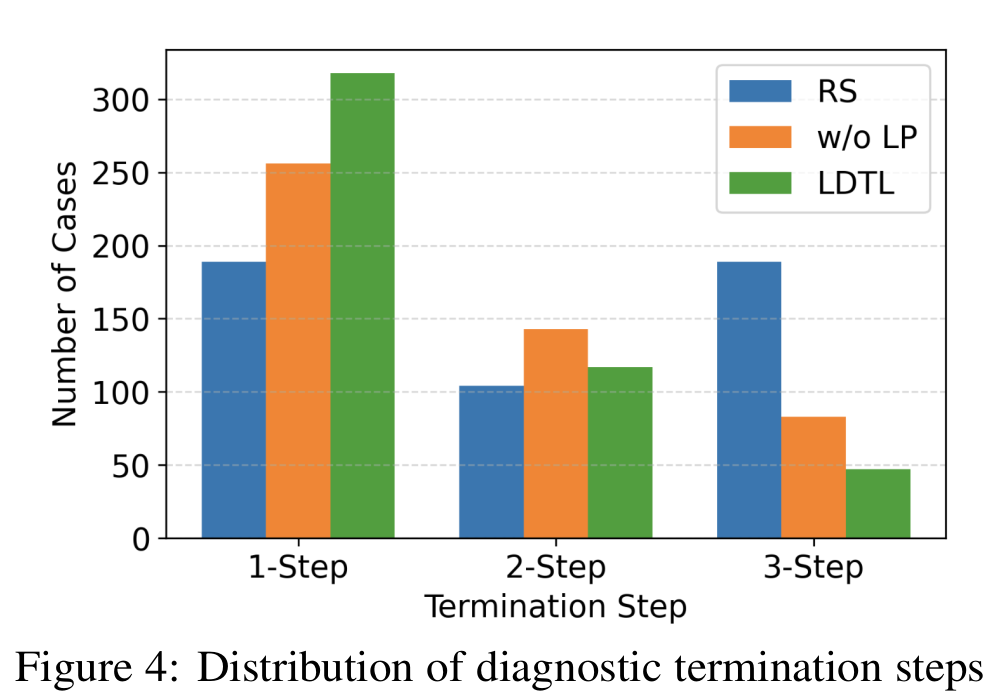
\includegraphics[
  width=0.80\linewidth,
  height=0.50\textheight,
  keepaspectratio,
  trim=0 0 0 0,
  clip
]{figures/LDTL/results/fig4_crop.png}
\end{frame}

\begin{frame}[plain]
\centering
\vspace{0.22\textheight}
{\Large\bfseries Learning What Matters: Criticality-Guided\\Reinforcement Learning for Sequential Clinical Diagnosis}
\vspace{1.2em}

{\small SIFT}\\
{\scriptsize Preprint 2026}
\end{frame}

\begin{frame}{SIFT: 문제 제기}
\vspace{0.1em}
\begin{block}{1. 기존 benchmark는 action과 diagnosis를 닫힌 공간으로 제한함}
\small
AMIE, ED-Copilot, LA-CDM 계열은 action space를 predefined test menu로 제한하고, diagnosis space도 fixed label set으로 둔다. 반면 실제 clinical reasoning은 open-ended interaction에 가깝다.
\end{block}

\vspace{0.45em}
\begin{block}{2. Terminal reward는 evidence quality를 보지 못함}
\small
최종 diagnosis가 맞았는지는 알려주지만, trajectory가 모은 evidence가 좋은지는 말해주지 않는다. 그래서 policy가 critical finding과 noise를 구분하지 못하고 \textbf{indiscriminate information acquisition}으로 흐를 수 있다.
\end{block}

\vspace{0.45em}
\begin{block}{SIFT의 문제 설정}
\small
정답 path를 직접 만들기보다, trajectory가 \textbf{critical evidence}를 얼마나 회수했는지를 reward signal로 만든다.
\end{block}
\end{frame}

\begin{frame}[t]{SIFT: Main Figure}
\centering
\vspace{0.35em}

\includegraphics[width=0.98\linewidth,height=0.78\textheight,keepaspectratio]{figures/SIFT/main.png}
\end{frame}

\begin{frame}{SIFT: 사전 criticality scoring}
\vspace{0.1em}
\begin{columns}[T,onlytextwidth]
\begin{column}{0.45\textwidth}
\centering

\includegraphics[width=0.98\linewidth,height=0.72\textheight,keepaspectratio]{figures/SIFT/image.png}
\end{column}
\begin{column}{0.51\textwidth}
\vspace{0.4em}
{\large\bfseries\textcolor{primary}{1. Fact extraction}}

\vspace{0.35em}
{\small Training 전에 patient record \(M\)에서 atomic clinical facts를 추출한다.}

\vspace{0.15em}
{\small \(F=\phi(M)=\{f_1,\ldots,f_n\}\)}

\vspace{0.25em}
{\footnotesize 각 \(f_i\)는 lab value, imaging finding, physical exam result처럼 해석이 섞이지 않은 단일 observation이다.}

\vspace{1.0em}
{\large\bfseries\textcolor{primary}{2. Criticality scoring}}

\vspace{0.35em}
{\small \(w_f=\psi(f\mid d^{*},o_0),\quad w_f\in\{0,1,2,3\}\)}

\vspace{0.25em}
{\footnotesize gold diagnosis \(d^{*}\)와 initial presentation \(o_0\) 기준으로 각 fact가 얼마나 diagnosis를 confirm하는지 점수화한다.}

\vspace{1.0em}
{\large\bfseries\textcolor{primary}{Score meaning}}

\vspace{0.25em}
{\footnotesize
\begin{itemize}
  \item \(0\): diagnosis와 무관
  \item \(1\): supportive but non-specific evidence
  \item \(2\): significant evidence
  \item \(3\): hallmark / pathognomonic finding
\end{itemize}
Scoring은 offline으로 수행되어 rollout 중 \(\psi\)를 호출하지 않는다.
}
\end{column}
\end{columns}
\end{frame}

\begin{frame}{SIFT: 방법}
\vspace{0.35em}
{\large\bfseries\textcolor{primary}{1. 왜 terminal reward만으로 부족한가}}

\vspace{0.35em}
{\small
최종 diagnosis가 맞았는지만 보는 binary reward는 episode 끝에서만 관측된다. 어떤 action이 correct diagnosis에 기여했는지 알려주지 못하고, agent가 진단적으로 무관한 정보까지 넓게 수집하는 방향으로 흐를 수 있다.
}

\vspace{1.0em}
\begin{columns}[T,onlytextwidth]
\begin{column}{0.48\textwidth}
{\large\bfseries\textcolor{primary}{2. Critical recall}}

\vspace{0.35em}
{\small
Trajectory가 회수한 critical facts의 비율을 측정한다.
}
\[
CR(\tau)=
\frac{\sum_{f \in D(\tau)} w_f}
{\sum_{f \in F} w_f}
\]
\vspace{-0.25em}
{\footnotesize \(F\): 전체 fact set, \(D(\tau)\): 발견된 fact set, \(w_f\): criticality score.}
\end{column}
\begin{column}{0.48\textwidth}
{\large\bfseries\textcolor{primary}{3. Criticality-weighted reward}}

\vspace{0.35em}
{\small
정답 여부와 critical evidence 회수를 같이 reward에 반영한다.
}
\[
R(\tau)=(\alpha CR(\tau)+\beta)\,\mathrm{acc}(\hat d,d^{*})
+\eta CR(\tau)-\lambda\frac{t}{T}
\]
\vspace{-0.25em}
{\footnotesize 같은 diagnosis accuracy라도 critical evidence를 더 많이 회수하면 reward가 커진다. 마지막 항은 step penalty다.}
\end{column}
\end{columns}
\end{frame}

\begin{frame}[t]{SIFT: 결과와 의미}
\centering
\vspace{0.25em}
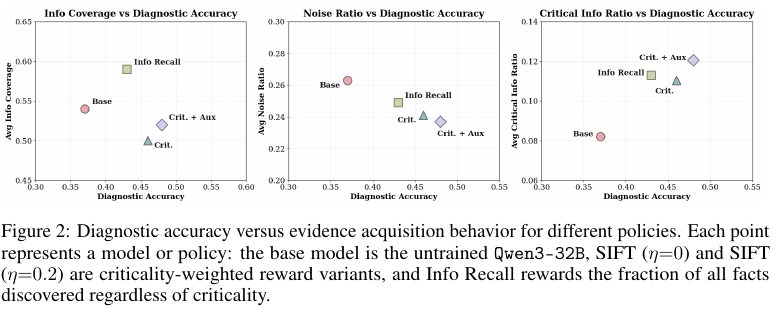
\includegraphics[width=0.98\linewidth,height=0.51\textheight,keepaspectratio]{figures/SIFT/result_evidence_quality.png}

\vspace{0.3em}
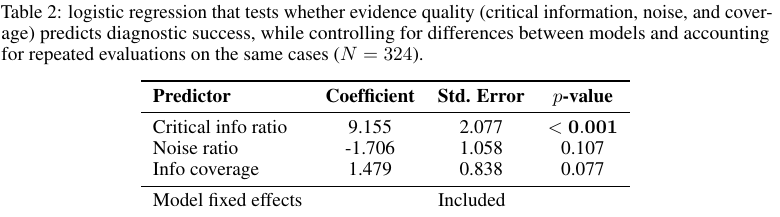
\includegraphics[width=0.76\linewidth,height=0.23\textheight,keepaspectratio]{figures/SIFT/result_logistic_regression.png}

\vspace{0.15em}
{\footnotesize 결과 해석: evidence의 양보다 critical evidence ratio가 diagnostic success를 가장 강하게 설명한다.}
\end{frame}

\begin{frame}{왜 trajectory를 모델링해야 할까? = 왜 greedy가 실패하나?}
\vspace{0.35em}
\begin{block}{핵심 문제}
\small
좋은 diagnostic path에는 정답 label이 없다. 그래서 기존 연구들은 terminal reward, local information gain, critical fact recall 같은 proxy를 만든다.
\end{block}

\vspace{0.35em}
\begin{columns}[T,onlytextwidth]
\begin{column}{0.48\textwidth}
{\large\bfseries\textcolor{primary}{Greedy가 아는 것}}

\vspace{0.35em}
{\small
현재 state \(S\)에서 action \(a\) 하나를 추가했을 때의 즉시 변화만 본다.
}
\[
\Delta U(a\mid S)=U(S\cup\{a\})-U(S)
\]
\vspace{-0.2em}
{\footnotesize 이 값이 크면 지금 당장은 좋아 보인다.}
\end{column}
\begin{column}{0.48\textwidth}
{\large\bfseries\textcolor{primary}{Greedy가 모르는 것}}

\vspace{0.35em}
{\small
그 action이 이후 어떤 검사 조합을 열어주는지, 혹은 이미 얻은 정보와 얼마나 겹치는지는 보지 못한다.
}
\[
U(S\cup A\cup B)\neq U(S\cup A)+U(S\cup B)
\]
\vspace{-0.2em}
{\footnotesize synergy와 redundancy는 trajectory 전체에서 드러난다.}
\end{column}
\end{columns}

\vspace{0.45em}
\begin{alertblock}{정리}
\small
``중간 reward가 없어서 어렵다''는 반만 맞는 설명이다. 더 근본적인 문제는 \textbf{중간 reward를 무엇으로 정의해야 trajectory-level utility를 보존하는가}다.
\end{alertblock}
\end{frame}

\begin{frame}{Greedy가 실패하는 예시: combination effect}
\vspace{0.1em}
\begin{columns}[T,onlytextwidth]
\begin{column}{0.48\textwidth}
\centering
{\large\bfseries\textcolor{primary}{Example 1: same second test \(C\)}}

\vspace{0.25em}
\begin{tikzpicture}[
  node distance=1.1cm and 1.55cm,
  state/.style={draw, rounded corners=2pt, align=center, minimum width=1.55cm, minimum height=0.82cm, font=\scriptsize, fill=white},
  good/.style={draw=primary, very thick, fill=SoftOrange},
  better/.style={draw=secondary, very thick, fill=secondary!8},
  edge/.style={->, thick},
  gre/.style={->, very thick, primary},
  alt/.style={->, very thick, secondary}
]
\node[state] (s) {Initial\\\(U=0.00\)};
\node[state, good, below left=of s] (a) {\(A\)\\\(U=0.70\)};
\node[state, below right=of s] (b) {\(B\)\\\(U=0.50\)};
\node[state, below=of a] (ac) {\(A+C\)\\\(U=0.71\)};
\node[state, better, below=of b] (bc) {\(B+C\)\\\(U=0.80\)};
\draw[gre] (s) -- node[above left, font=\scriptsize] {\(A\)} (a);
\draw[edge] (s) -- node[above right, font=\scriptsize] {\(B\)} (b);
\draw[edge] (a) -- node[left, font=\scriptsize] {\(+C\)} (ac);
\draw[alt] (b) -- node[right, font=\scriptsize] {\(+C\)} (bc);
\end{tikzpicture}

\vspace{0.25em}
{\footnotesize
Greedy는 \(U(A)>U(B)\)라서 \(A\)를 고른다. 하지만 같은 \(C\)를 붙이면 \(B+C\)가 더 높다.
}
\end{column}
\begin{column}{0.48\textwidth}
\centering
{\large\bfseries\textcolor{primary}{Example 2: different second test}}

\vspace{0.25em}
\begin{tikzpicture}[
  node distance=1.1cm and 1.55cm,
  state/.style={draw, rounded corners=2pt, align=center, minimum width=1.55cm, minimum height=0.82cm, font=\scriptsize, fill=white},
  good/.style={draw=primary, very thick, fill=SoftOrange},
  better/.style={draw=secondary, very thick, fill=secondary!8},
  edge/.style={->, thick},
  gre/.style={->, very thick, primary},
  alt/.style={->, very thick, secondary}
]
\node[state] (s2) {Initial\\\(U=0.00\)};
\node[state, good, below left=of s2] (a2) {\(A\)\\\(U=0.70\)};
\node[state, below right=of s2] (b2) {\(B\)\\\(U=0.50\)};
\node[state, below=of a2] (ac2) {\(A+C\)\\\(U=0.72\)};
\node[state, better, below=of b2] (bd2) {\(B+D\)\\\(U=0.82\)};
\draw[gre] (s2) -- node[above left, font=\scriptsize] {\(A\)} (a2);
\draw[edge] (s2) -- node[above right, font=\scriptsize] {\(B\)} (b2);
\draw[edge] (a2) -- node[left, font=\scriptsize] {\(+C\)} (ac2);
\draw[alt] (b2) -- node[right, font=\scriptsize] {\(+D\)} (bd2);
\end{tikzpicture}

\vspace{0.25em}
{\footnotesize
처음엔 \(A\)가 더 좋아 보이지만, \(B\)가 \(D\)와 만나면 더 큰 trajectory utility를 만든다.
}
\end{column}
\end{columns}

\vspace{0.25em}
\begin{alertblock}{의미}
\small
이 현상은 검사 정보가 독립적이지 않다는 뜻이다. 한 검사의 가치는 단독 값이 아니라 \textbf{이후 어떤 검사와 결합되는지}에 따라 달라진다.
\end{alertblock}
\end{frame}

\end{document}
